\documentclass{patmorin}
\listfiles
\usepackage{amsthm,amsmath,graphicx,wrapfig}
\usepackage{pat}
%\usepackage{coffee4}
\usepackage[letterpaper]{hyperref}
\usepackage[dvipsnames]{color}
\definecolor{linkblue}{named}{Blue}
\hypersetup{colorlinks=true, linkcolor=linkblue,  anchorcolor=linkblue,
citecolor=linkblue, filecolor=linkblue, menucolor=linkblue, 
urlcolor=linkblue, pdfcreator=Me, pdfproducer=Me} \setlength{\parskip}{1ex}

\title{\MakeUppercase{Fourth Workshop on Geometry and Graphs:
       Open Problems}}
\author{Bellairs 2016}


%\usepackage{lineno}
%\linenumbers

\begin{document}
\begin{titlepage}
\maketitle

\begin{abstract}
  A collection of open problems posed by participants of and studied at
  the Fourth Workshop on Geometry and Graphs.
\end{abstract}
\end{titlepage}

\pagenumbering{roman}
\tableofcontents
\newpage

\pagenumbering{arabic}


\section{A Grid Puzzle}

\noindent\emph{Pat Morin}

Consider the following game/puzzle played on the $n\times n$ integer
grid $G=\{(i,j):i,j\in\{1,\ldots,n\}\}$.  Initially, all points in $G$
are marked as \emph{live}.  

The game proceeds in $n$
rounds. During the $i$th round, the player selects a monotonically
increasing set, $P_i$, of live points in $G$.\footnote{Here monotonically
increasing means that each point in $P_i$ has a unique $x$-coordinate
and $y$-coordinate and, for every $(i_1,j_1),(i_2,j_2)\in P_i$, $i_1 <
i_2\Leftrightarrow j_1<j_2$.}  Each point $(i,j)$ selected in $P_i$
\emph{kills} the L-shape $\{(i,j'): j'\ge j\}\cup\{(i',j):i'\ge i\}$ so 
that these points are no longer live in subsequent rounds. 

The game ends after $n$ rounds and the player's score is $\sum_{j=1}^n |P_i|$.

\begin{op}
   What is the maximum score a player can earn in this game?
\end{op}

By playing a cluster of $\sqrt{n}$ points in each round starting with a cluster
in the top-right corner, a player can earn a score of $\Omega(n^{3/2})$: 

\begin{center}
   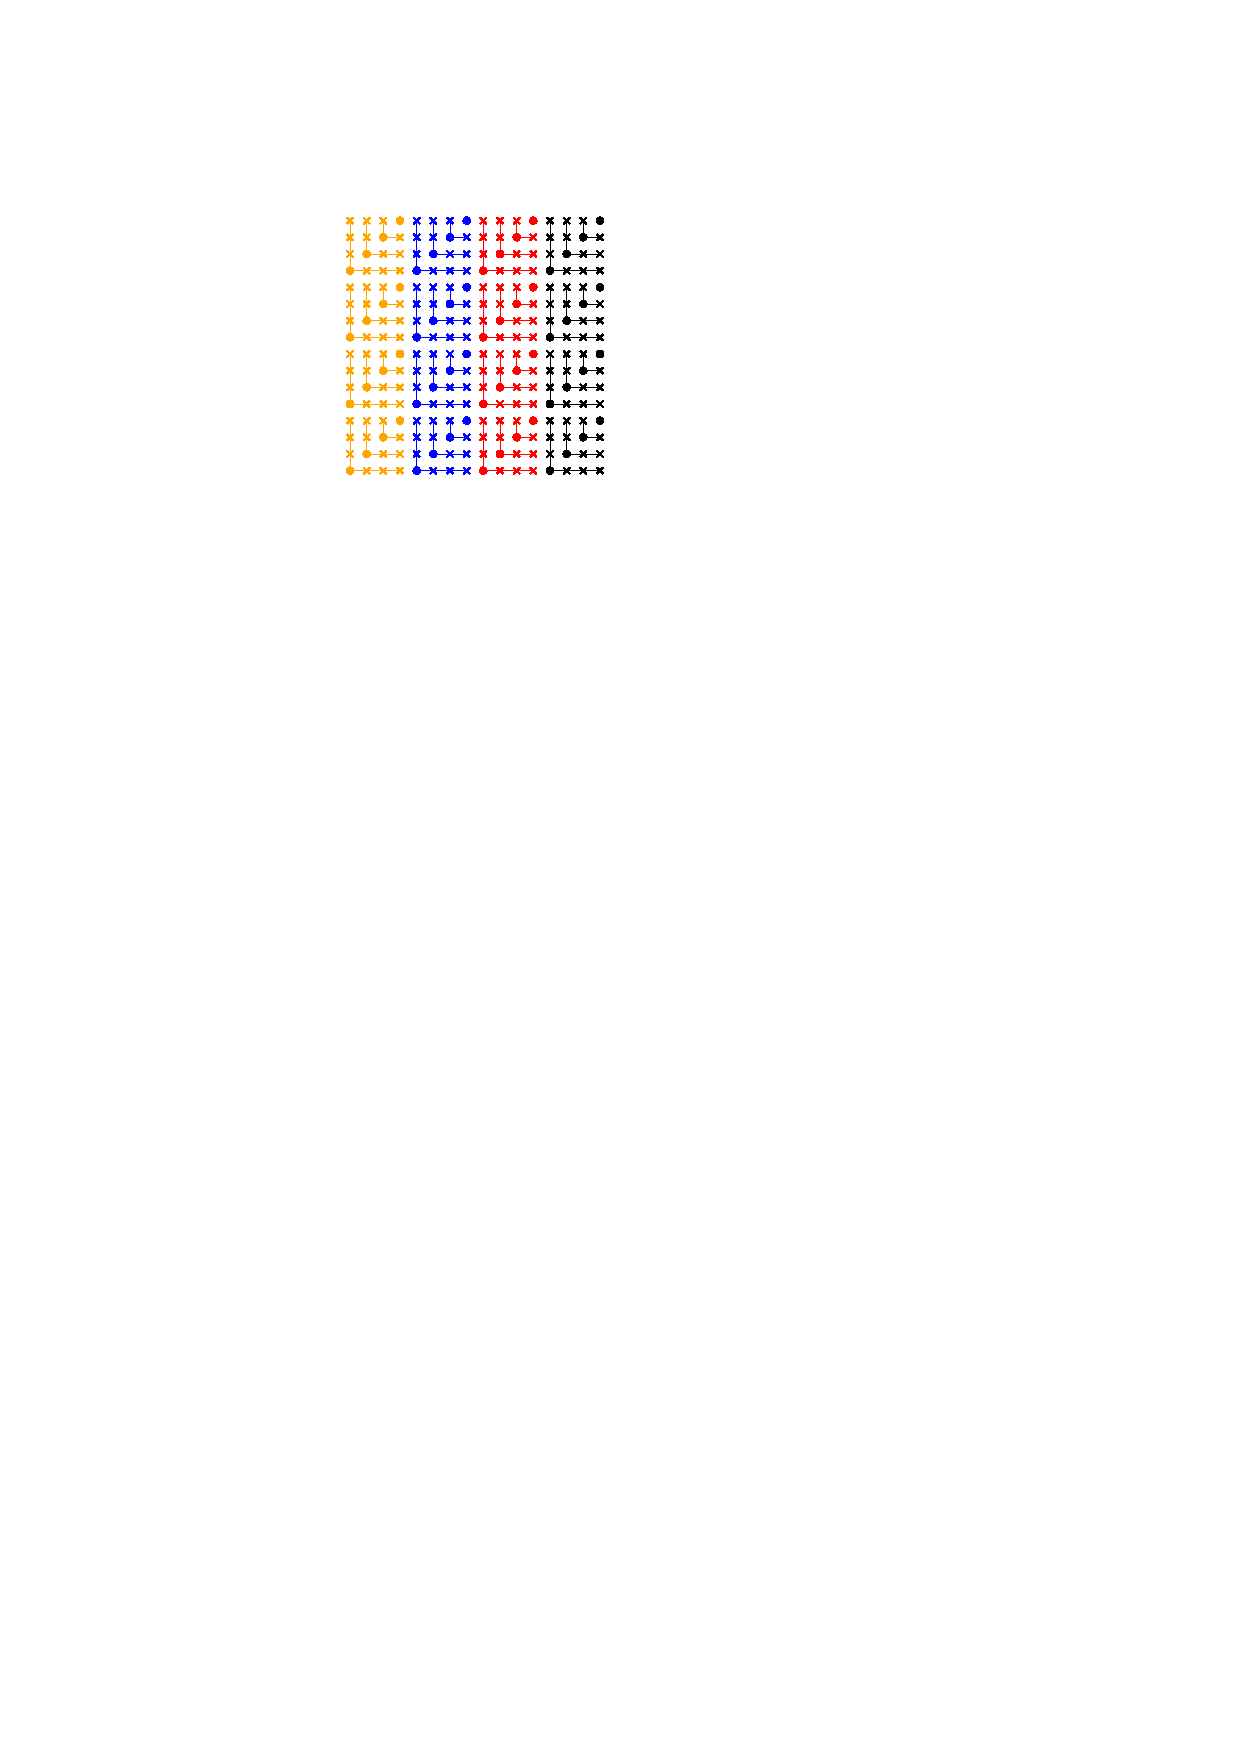
\includegraphics{figs/game}
\end{center}

This seems optimal, but I've been unable to prove it.

\noindent History: this game models a combinatorial geometry problem
posed by Bra\ss\ (2004) of determining the maximum number of triangles
one can draw on a convex point set before creating a pair of triangles
that (a)~share an edge and cross or (b)~share a vertex but whose edges
oppposite the shared vertex do not cross.

\section{Facial Nonrepetitive Colouring of Trees}

\noindent\emph{Vida Dujmovi\'c}

A non-empty even-length sequence $S$ is a \emph{repetition} if it is the
concatenation of two equal non-empty sequences; in other words, $S$ is
a repetition if $S=RR$ for some non-empty sequence $R$.  A \emph{block}
in a sequence is a non-empty contiguous subsequence.  A sequence $S$ is
\emph{nonrepetitive} if none of its blocks is a repetition. (Nonrepetitive
sequences are also sometimes called \emph{square free} since they have
no block of the form $RR=R^2$.)

A classic result of Thue, from 1906, states that there are arbitrarily
long nonrepetitive sequences on an alphabet of size 3.  This notion has
been generalized to graph colourings, where we say that a colouring of
a graph $G$ is \emph{nonrepetitive} if, for every (simple) path, $P$,
in $G$, the sequence of $P$'s colours is not a repetition.

This question asks about nonrepetitive colourings of trees.  It is known
that every tree has a nonrepetitive 4-colouring and that this is optimal
for some trees. Here is a warm-up question, that would only need a slight
generalization of Thue's result:

\begin{op}
  Let $T^3_n$ be the tree having one vertex of degree 3 attached to three
  paths of length $n$.  Does $T^3_n$ have a nonrepetitive 3-colouring?
\end{op}

A \emph{facial path} in an embedded graph, $G$, is a path that appears
as a block in the facial walk of some face of $G$.  A \emph{facial
nonrepetitive colouring} of $G$ is a colouring where, for each facial
path, $P$, of $G$, the sequence of colours encountered in $P$ is not
a repetition. It is known, for example, that every plane graph has a
facial nonrepetitive 22-colouring.

\begin{op}\oplabel{facial-tree-colouring}
  Does every (ordered) tree have a facial nonrepetitive 3-colouring? 
\end{op}

Note that the facial nonrepetitive 22-colouring of plane graphs
uses nonrepetitive colouring of trees as a building block (twice), so
solving \opref{facial-tree-colouring} would give a facial nonrepetitive
20-colouring of plane graphs.

\section{Optimal isotopic embedding}

\noindent\emph{G\"unter Rote}

We are given a (small) undirected \emph{guest graph} $G=(V_0,E_0)$
and a larger undirected \emph{host graph} $H=(V,E)$.
Both graphs are embedded in the plane.
We look for an isotopic embedding from $G$ to $H$ with
a given vertex assignment $V_0\mapsto V$. This means that
the edges $e\in E_0$ have to be mapped to edge-disjoint
paths $p(e)$ in $H$ such that the resulting image of $p(G)$ is obtained
from $G$ by a deformation of the plane. The face structure, orientation,
etc.\ of $G$ must be preserved, except that different edges $p(e)$
and $p(e')$ are allowed to ``touch'' (but not cross) at vertices.
(As an alternative, we might also ask for vertex-disjoint embeddings of edges.)

In addition, we are given a nonnegative cost function
$c_e\colon E\to R$, separately for each edge $e\in E_0$ that is to be embedded.
The objective is to minimize the total cost
$\sum_{e\in E_0} \sum_{f \in p(e)} c_e(f)$.

What is the complexity of this problem for small fixed
graphs $G$? For example, when $G$ is a triangle?

When $|V_0|=2$ and $G$ consists just of parallel edges,

I can model the problem as a dual network flow problem and solve it
in polynomial time.

\section{Straightening monotone drawings}

\noindent\emph{G\"unter Rote}

We are given a plane drawing of a graph where every
edge is both $x$-monotone and $y$-monotone.
\begin{op}
Can such a drawing always be straightened in such a way
that the edges are $x$-monotone and $y$-monotone
in the same sense as before?
\end{op}
It is know than it can be done with at most one bend per edge.

\section{Free edge in planar UDGs}

\noindent\emph{Ahmad Biniaz}

A \emph{free edge} in a unit disk graph is an edge which is not
intersected by other edges. There are some UDGs that have no free
edge. The question is:

\begin{op}
  Does any planar UDG have a free edge?
\end{op}

\noindent (Note the qualifier \emph{planar} (as opposed to \emph{plane}) in the
preceding problem.)


\section{Plane Red Blue Matchings}

\noindent\emph{Ahmad Biniaz}

We have a set $R$ of red points and a set $B$ of blue points in the plane such that ($R\cup B$) is in general position and $|R|+|B|$ is a big number. We want to match the red points together and the blue points together so that the union of these two matchings is non-crossing. It may not be possible to compute a perfect non-crossing matching even if both $|R|$ and $|B|$ are even numbers. In 2001, Dumitrescu and Kaye [1] showed that it is possible to match $85.71\%$ of the total number of points. They also showed there are large point sets which do not admit a plane matching which matches more than $98.95\%$ of the points. 

\begin{op}
  Improve these lower and upper bounds.
\end{op}

\noindent
Adrian Dumitrescu, Rick Kaye: Matching colored points in the plane: Some new results. Comput. Geom. 19(1): 69-85 (2001)

\section{Grid point sets with no convex $n$-gons}

\noindent\emph{Ruy Fabila}

\begin{op}
  Does there exist, for every $\gamma \ge 1$ and every $n >0$, a suitable constant $\varepsilon(\gamma)>0$ and a set $S$
  of $n$ points in general position in the plane
  with the following property:
 $S$ has positive integer coordinates not exceeding $n^\gamma$, and $S$ does not contain a convex $\varepsilon(\gamma)\log_2(n)$-gon?
\end{op}

\begin{op}\label{prob:int_empty}
 Does the following holds for every constant $\gamma \ge 0$? 
 Every sufficiently large set of $n$ points in the general position in the plane with positive integer coordinates that do not exceed
 $n^{\gamma}$ contains an empty convex $7$-gon.
\end{op}

\section{Packing and covering $K_4$'s in a graph}

\noindent\emph{Abdul Basit}

Given a graph $G$, we would like to make $G$ $K_4$-free by deleting a
small number of edges. An obvious approach to do this is the following:
Let $F$ be a maximal family of pairwise edge disjoint $K_4$'s in
$G$. Clearly we need to delete at least one edge from every element of
$F$, and it suffices to delete all edges from every element of $F$. Let
$\nu(G)$ be the maximum size of an edge-disjoint family of $K_4$'s in
$G$, and $\tau(G)$ be the minimum number of edges required to delete
every $K_4$ in $G$. The above argument shows that $\nu(G) \leq \tau(G)
\leq {4 \choose 2} \nu(G)$. The lower bound is sharp, as seen by taking
$G$ to be the disjoint union of $K_4$'s. Taking $G$ to be $K_8$ shows
that $\tau(G)$ can be as large as $3.5 \nu(G)$.

\begin{op}
Does there exist a constant $c$ such that $\tau(G) \leq ({4 \choose 2}
- c) \nu(G)$?
\end{op}


\section{Minimal Rectangle Tilings}

\noindent\emph{Andrew Winslow}

Klarner [1969] defined the \emph{order} of a polyomino to be the smallest number of copies that tile a rectangle. Polyominoes with order $4s$ are known for all $s$ [Golomb 1989], as well as a small number of other even orders [Marshall 1997]. It was proved that no polyomino has order 3 [Stewart, Wormstein 1992] using a long case analysis, but results for larger odd n remain open:

\begin{op}
Does there exist a polyomino with odd order $n > 3$?
\end{op}

\begin{center}
  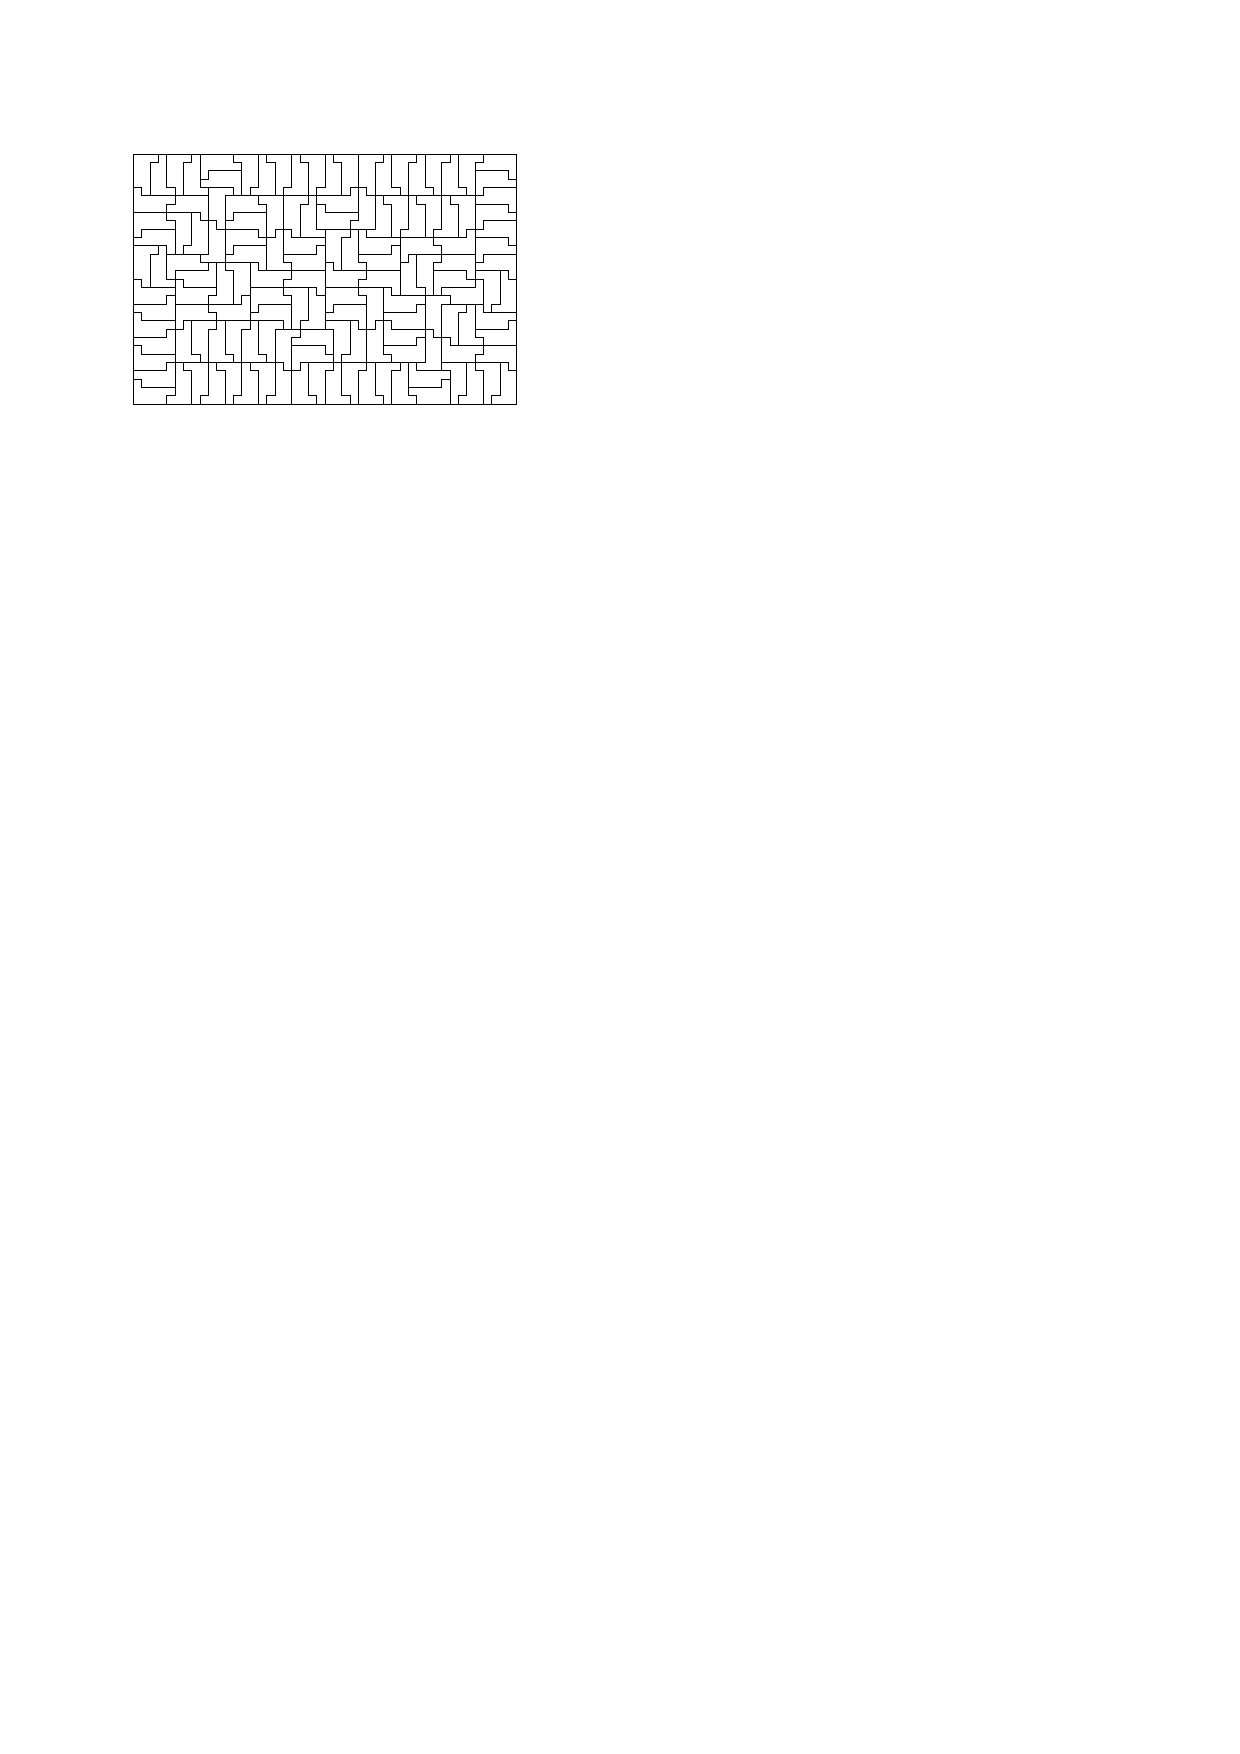
\includegraphics{figs/tiling.pdf}\\
  {The smallest rectangle tiled by this polyomino (of order 138).}
\end{center}

A similar problem has been considered for general polygons. For every prime number $n$, a square can be tiled using $n$ congruent copies of a polygon using rectangles arranged in a single column. In the 1980s, Danzer conjectured that no other tilings exist; this conjecture was confirmed for $n = 3$ [Maltby 1994] and $n = 5$ for the special case of convex polygons [Yuan, Zamfirescu, Zamfirescu 2016].

\begin{op}
Does there exist a tiling of a square using a prime number of congruent copies of a non-rectangular polygon?
\end{op}

\section{Approximation Algorithms for Slope Number}

The slope number of a graph is the minimum number of slopes of edges
needed in a drawing of the graph, with the edges drawn as straight line
segments, but allowing edges to cross. It is known that the slope number
is at least $\Delta/2$, where $\Delta$ is the maximum degree, but that
there exist bounded-degree graphs with unbounded slope number. It is
also known that planar graphs of bounded degree have bounded slope number
(exponential in the degree) and that testing whether the slope number is
two is NP-complete. It remains NP-complete for testing whether a planar
graph has a planar drawing with slope number two.

\begin{op}
  What can we say about approximating the slope number, either of all
  graphs, of all planar drawings of planar graphs, or of some interesting
  subclasses of graphs. Are there graph classes with unbounded slope number
  for which we can approximate this number accurately? Alternatively,
  can we prove any inapproximability results for slope number?
\end{op}

\end{document}


